\chapter{Experimental Results}
\section{Scanning procedure}
In order to evaluate the performance of the platform, several scans of the author's room at the student dormitory were performed.
The angular spacing between consecutive platform positions was set to \SI{0.8}{\degree}. With this setting, the total scanning time was approximately two minutes.

A video showing the scanning procedure is available at \href{https://youtube.com/shorts/UBePfZQdfIo?feature=share}{this link}.
A screen recording of the Open3D visualisation of the point cloud being built in real time is available at \href{https://youtu.be/SptaiVY_dwU}{this link}.

\section{Point Cloud Processing}
\subsection{Outlier Removal}
The obtained raw point cloud is shown in \cref{fig:raw_scan}.
The overall boxy shape of the room is already visible; however, many spurious points can be seen far away from the scanned environment.
These points are a result of faulty \gls{lidar} measurements.


Since these faulty measurements are spatially separated from the main point cloud, they can be removed using outlier filtering tools provided by Open3D\footnote{Link: \url{https://www.open3d.org/docs/release/tutorial/geometry/pointcloud_outlier_removal.html}}.
\begin{figure}[H]
    \centering
    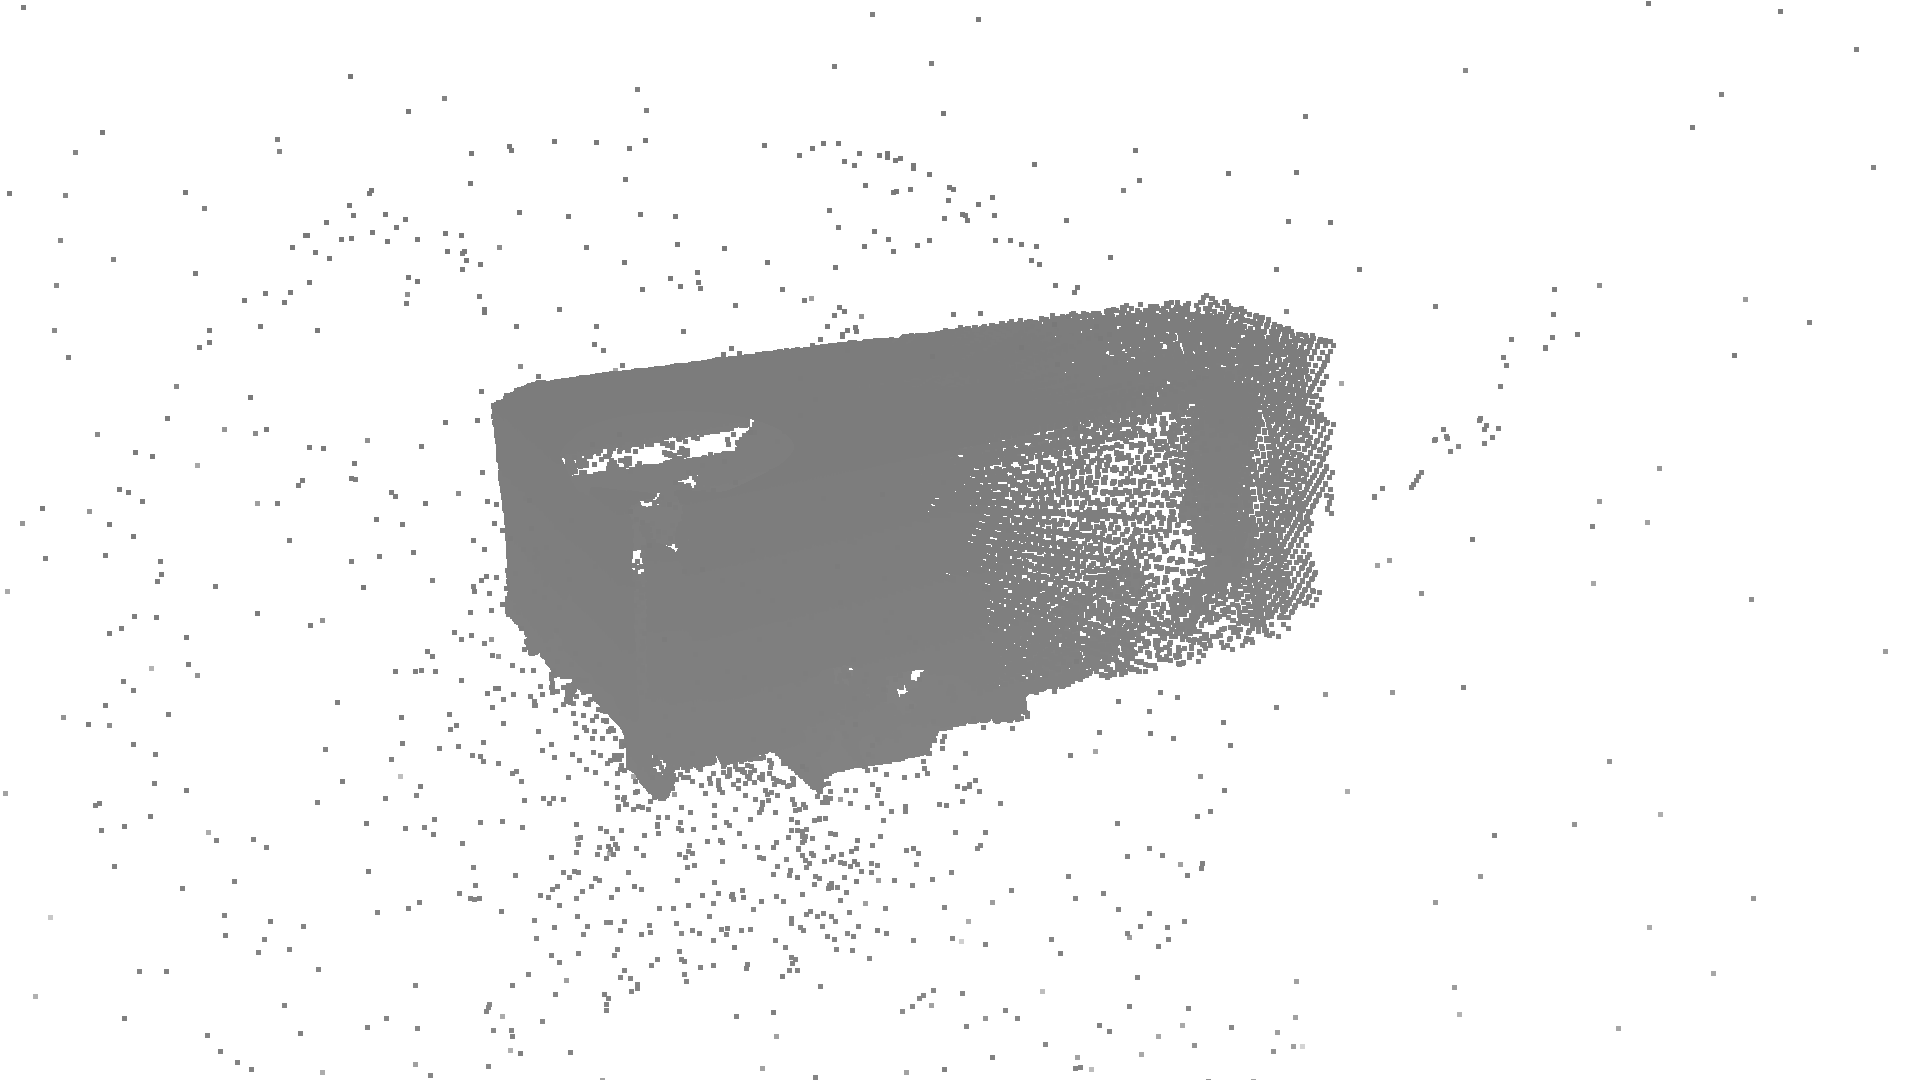
\includegraphics[width=\linewidth]{experimental_results/photos/z_raw_pcd.png}
    \caption{Raw point cloud}
    \label{fig:raw_scan}
\end{figure}

\begin{figure}[H]
    \centering
    \begin{subfigure}{0.90\linewidth}
        \centering
        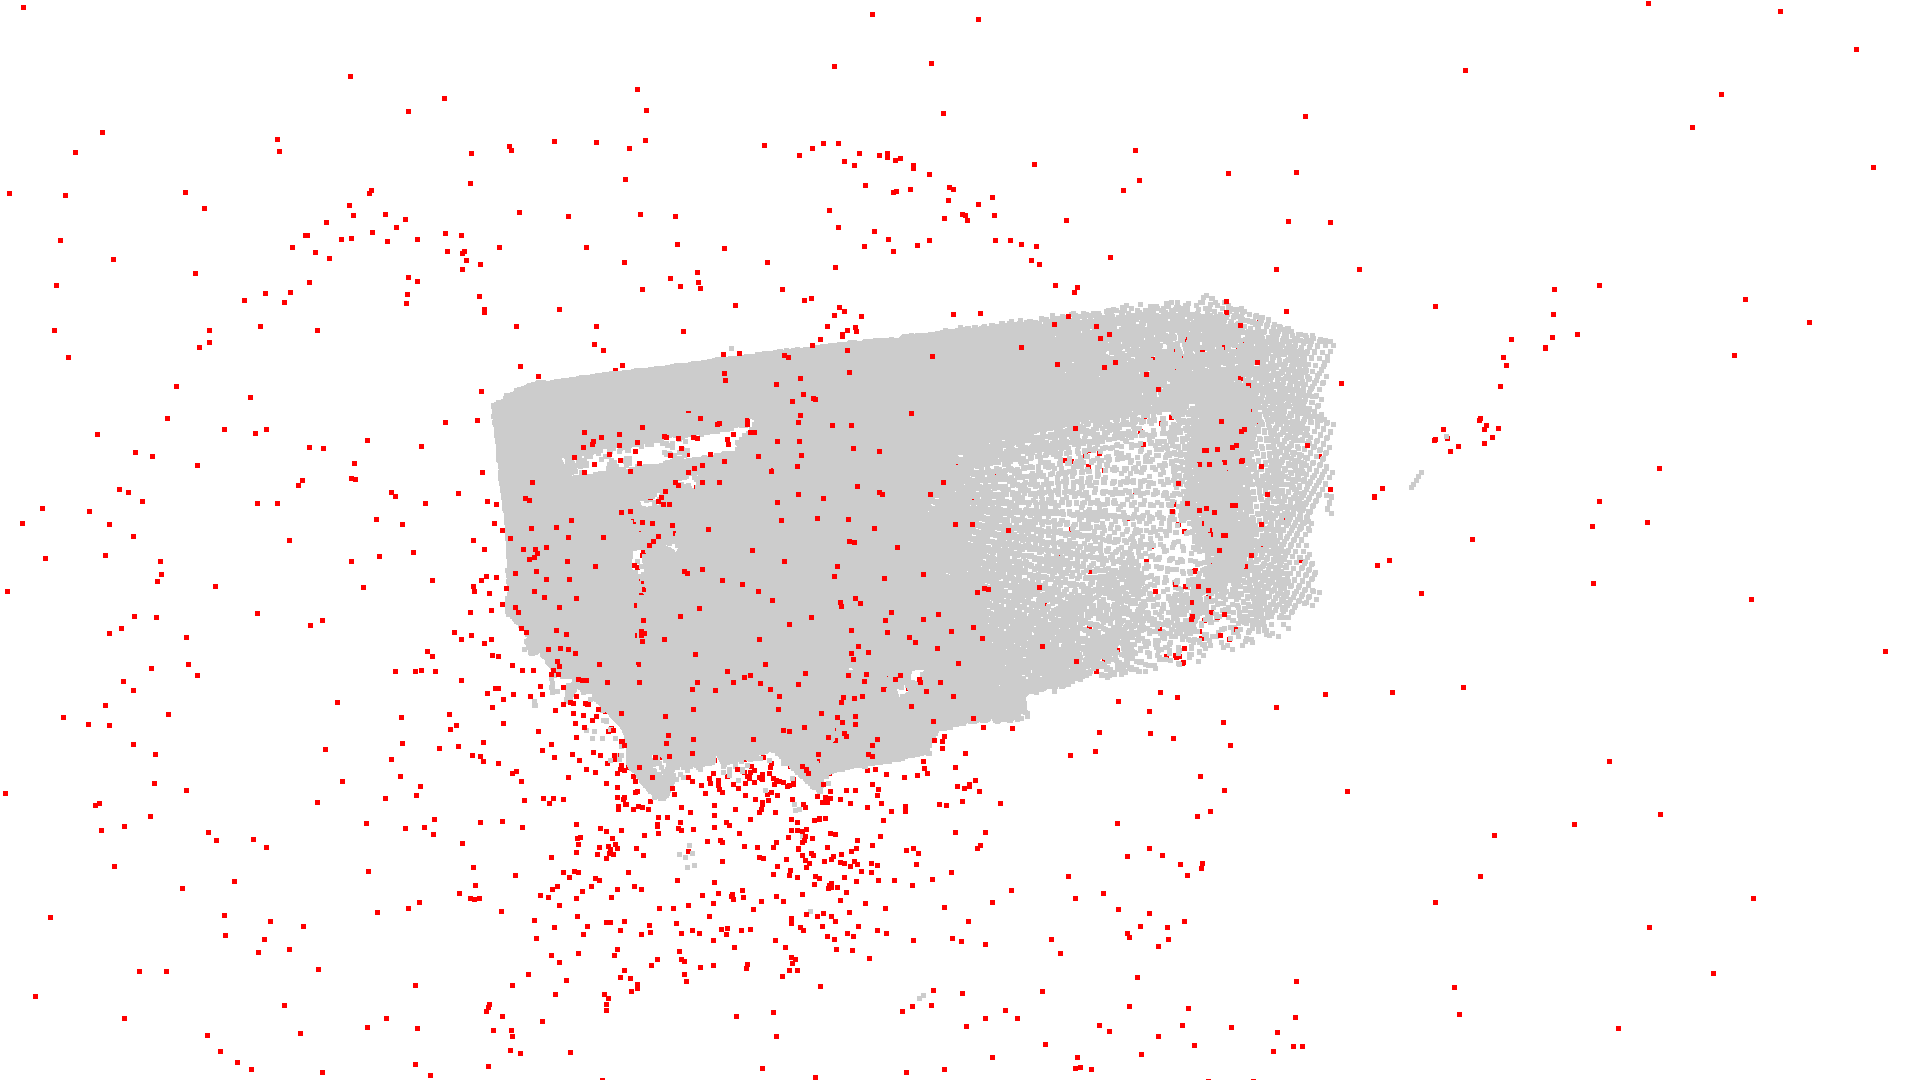
\includegraphics[width=\linewidth]{experimental_results/photos/z_outlier_delete.png}
        \caption{Red points are going to be removed}
    \end{subfigure}
    \hfill
    \begin{subfigure}{0.70\linewidth}
        \centering
        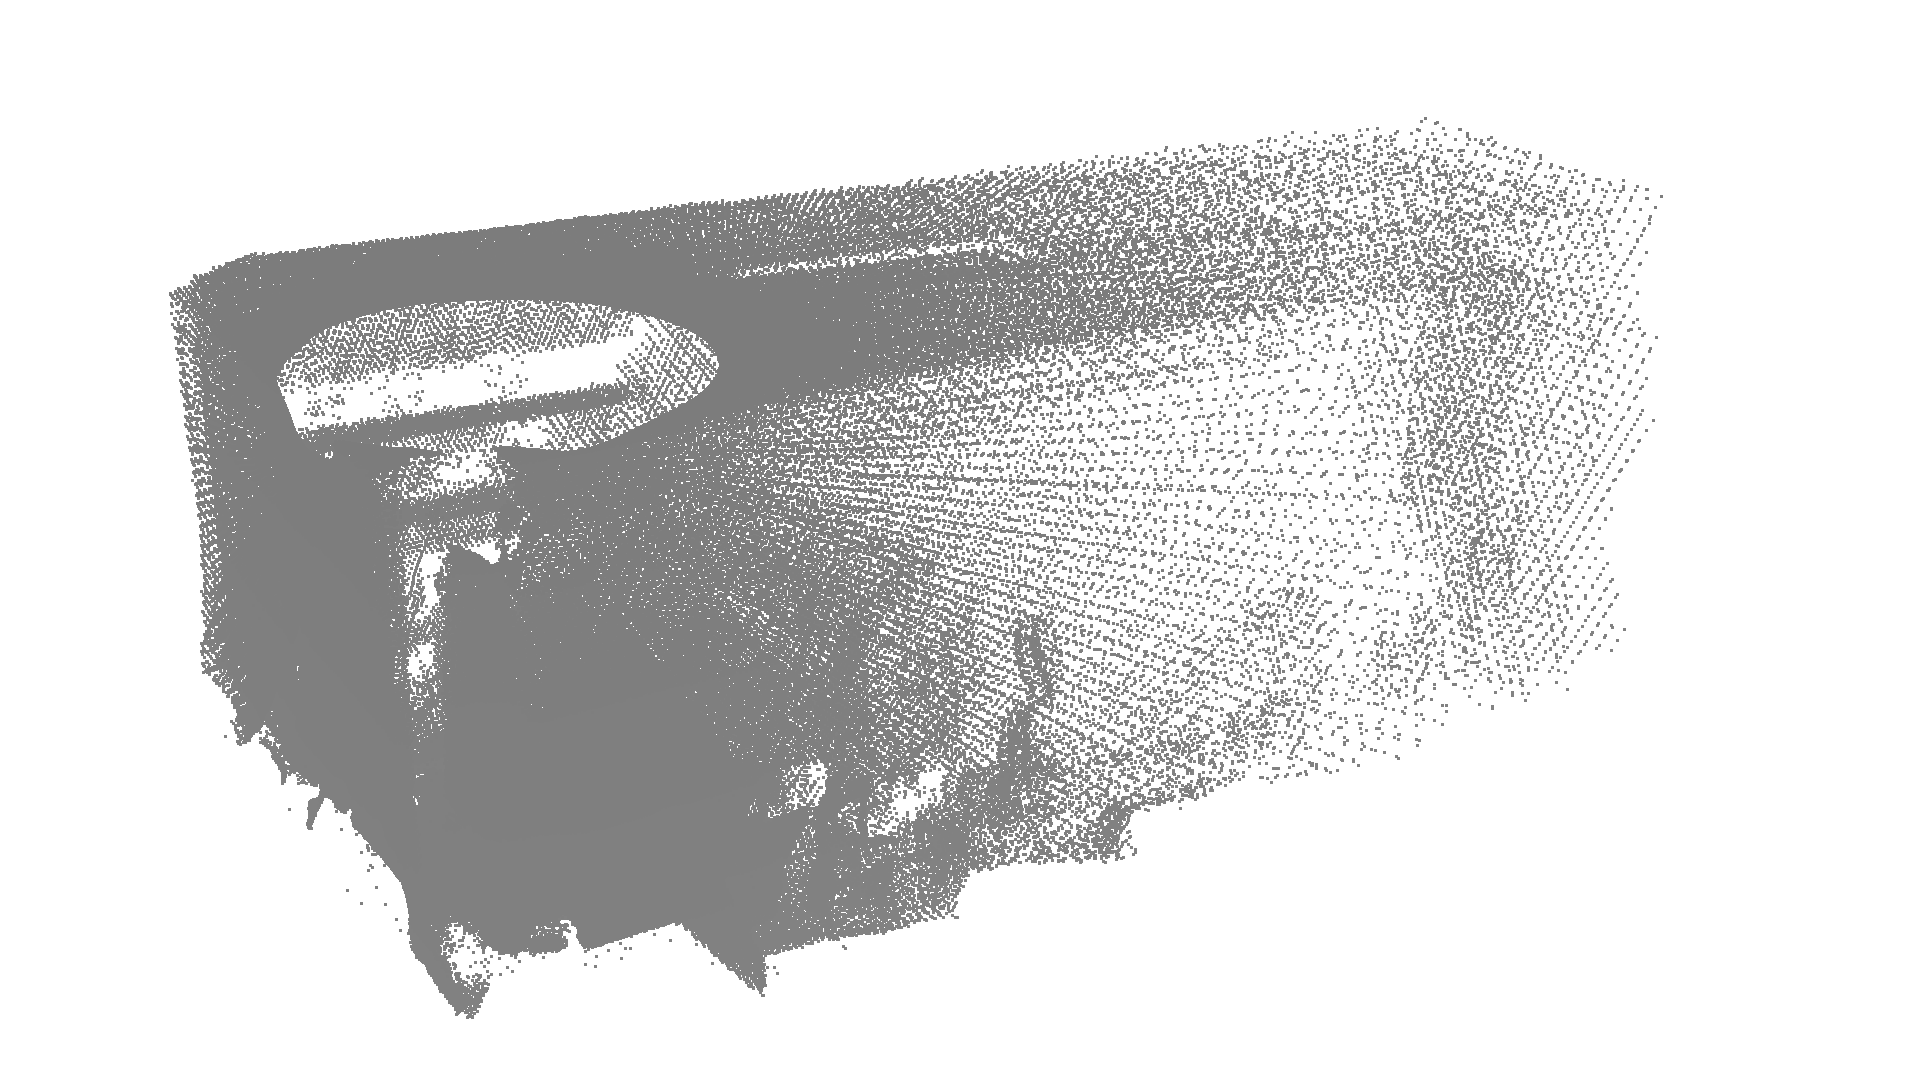
\includegraphics[width=\linewidth]{experimental_results/photos/z_outlier_show.png}
        \caption{Filtered point cloud}
    \end{subfigure}
    \caption{Visualisation of the outlier removal process}
\end{figure}

\subsection{Misalignment Corrections}
After filtering, misalignments between individual scan slices became visible. 
These misalignments were most noticeable at wide planes, such as the ceiling and the walls and were made by the reconstruction from \gls{lidar} scan slices acquired at platform azimuth angles differing by \SI{180}{\degree}.
The exact cause of these misalignments is not known; however, two possible explanations are proposed, each of which was corrected separately.

The first correction was aimed at the misalignment of the ceiling.
The mathematical transformation presented at \cref{subsec:point_cloud_reconstruction} assumes the x-axis of internal coordinate system of the \gls{lidar} sensor to be perfectly horizontal.
However, it is possible that the holes on the platform used for mounting the sensor were not perfectly level, causing a small angular error in the orientation of the sensor.
To compensate for this effect, an experimental correction of \SI{-1,0}{\degree} was found to produce the best alignment of the ceiling when applied to every acquired scan slice before the tilt transformation.

\begin{listing}[H]
\caption{Code snippet with the compensation for assumed \gls{lidar} misalignment}
\begin{minted}[linenos, frame=single, breaklines]{python}
    def lidarTo3D(distance_mm, scan_angle_deg, azimuth_deg):
        r = distance_mm/1000. # mm -> m
        scan_angle_rad = np.deg2rad(scan_angle_deg-1.0) ### correction of the possible lidar misalignment ###
        tilt = np.deg2rad(PLATFORM_TILT_DEG)
        azimuth_rad = np.deg2rad(azimuth_deg)

        # lidar local 2d plane
        x = r*np.cos(scan_angle_rad)
        y = r*np.sin(scan_angle_rad)
        z = 0 

        # tilt around x axis
        x_t = x
        y_t = y * np.cos(tilt) - z * np.sin(tilt)
        z_t = y * np.sin(tilt) + z * np.cos(tilt)

        # azimuth rotation around z
        x_a = x_t * np.cos(azimuth_rad) - y_t * np.sin(azimuth_rad)
        y_a = x_t * np.sin(azimuth_rad) + y_t * np.cos(azimuth_rad)
        z_a = z_t
        return [x_a,y_a,z_a]
\end{minted}
\end{listing}

\begin{figure}[H]
    \centering
    \begin{subfigure}{\linewidth}
        \centering
        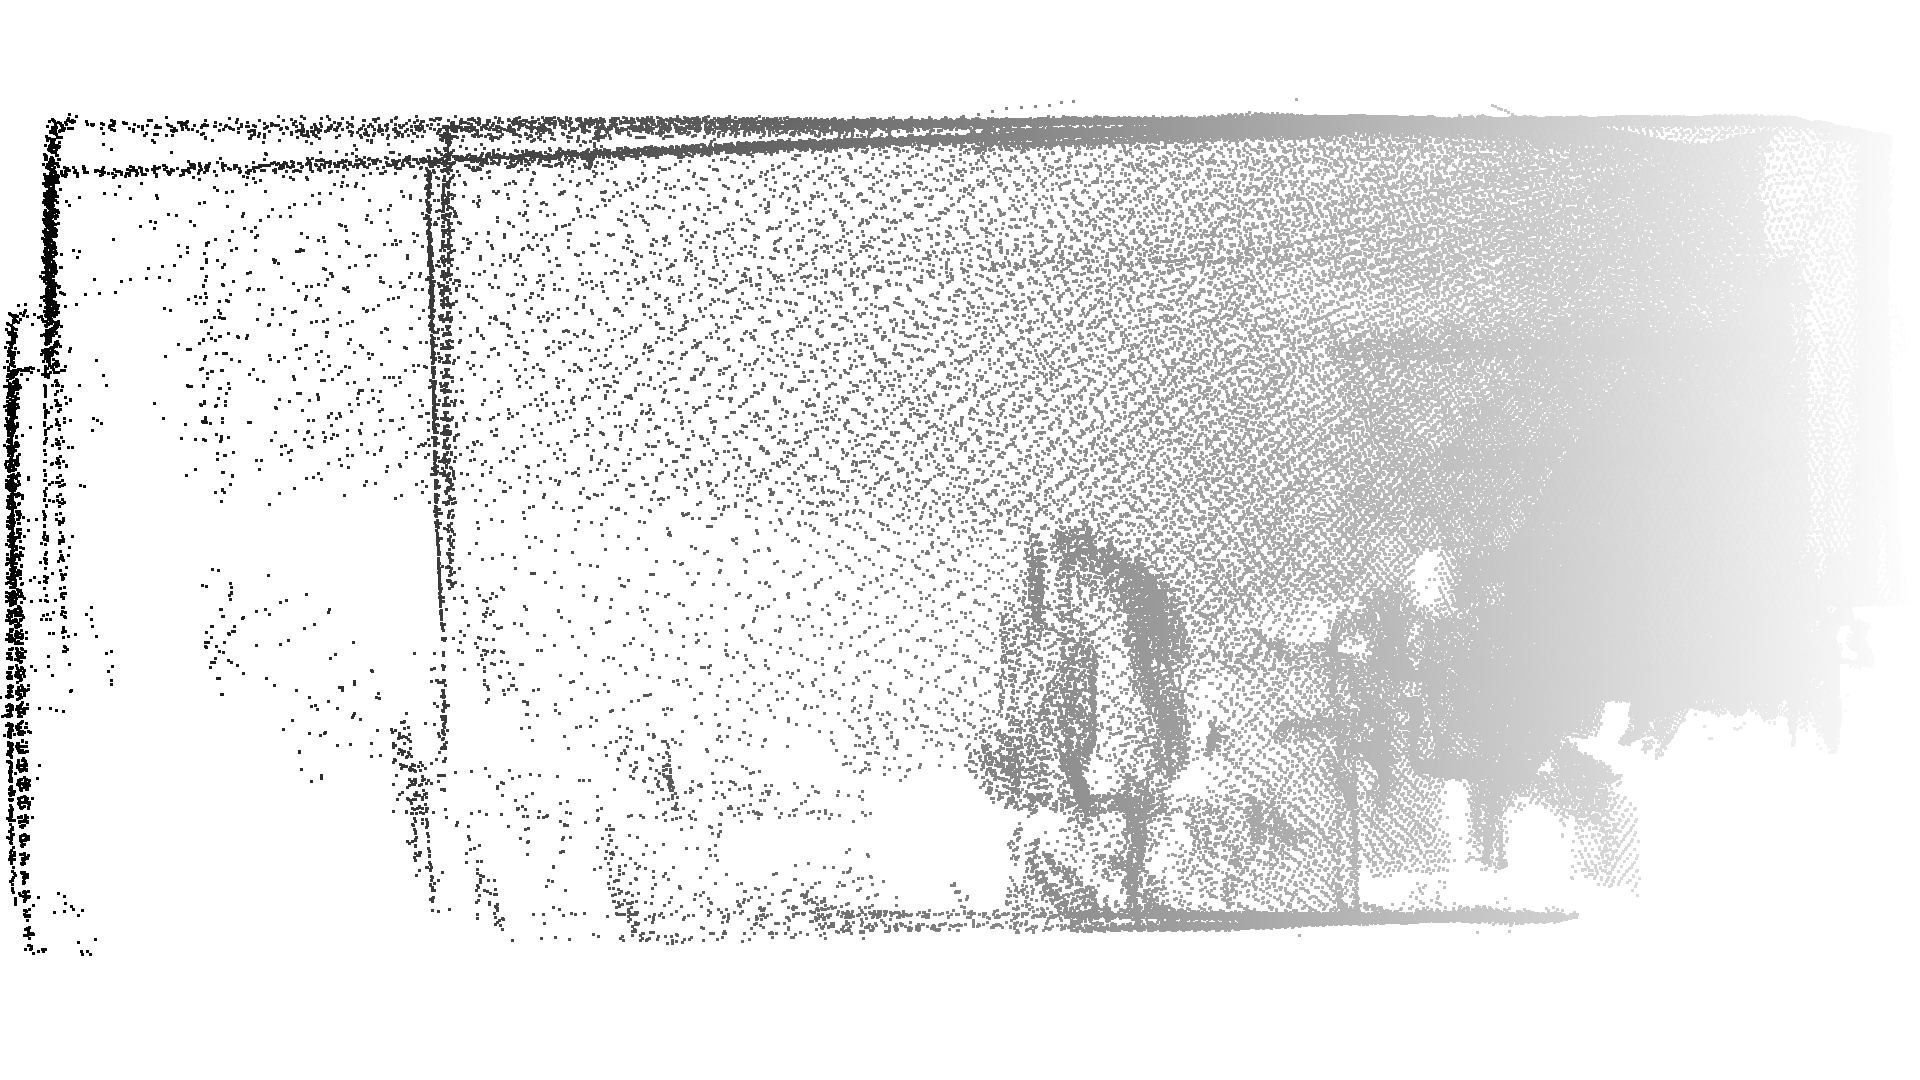
\includegraphics[width=\linewidth]{experimental_results/photos/z_bad_ceiling_grayscale.png}
        \caption{Before correction}
    \end{subfigure}
    \hfill
    \begin{subfigure}{\linewidth}
        \centering
        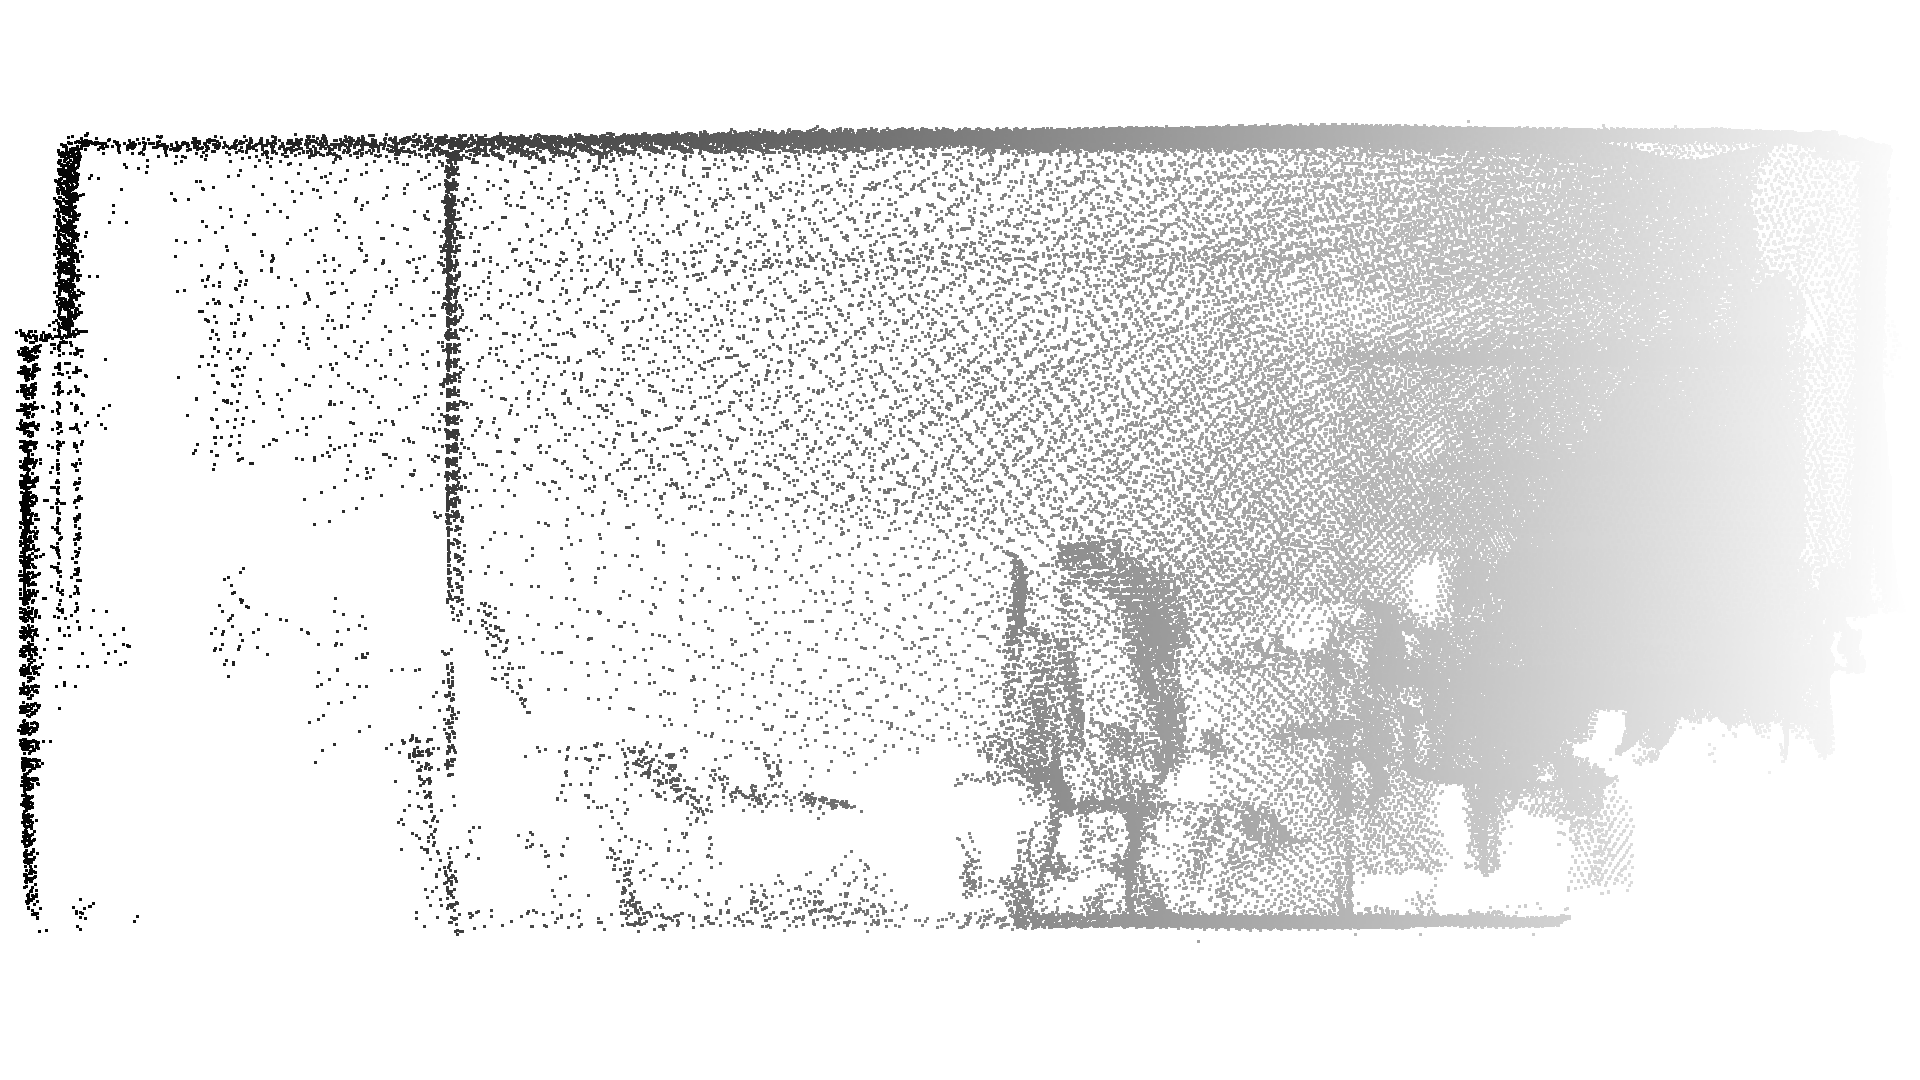
\includegraphics[width=\linewidth]{experimental_results/photos/z_good_ceiling_grayscale.png}
        \caption{After correction}
    \end{subfigure}
    \caption{Correction of the ceiling misalignment shown in side view}
\end{figure}

The second correction was aimed at the misalignment of walls.
It was assumed that the LiDAR beam was not emitted exactly in the expected local plane, rather at a small vertical angle.
This means that an acquired slice is not a slice but a collection of points shifted up vertically by an amount proportional to the measured distance.
An experimental correction of \SI{1,5}{\degree} was found to produce the best alignment of the walls when applied before the tilt transformation.

\begin{listing}[H]
\caption{Code snippet containing two corrections\protect\footnotemark}
\begin{minted}[linenos, frame=single, breaklines]{python}
def lidarTo3D(distance_mm, scan_angle_deg, azimuth_deg):
    r = distance_mm/1000. # mm -> m
    scan_angle_rad = np.deg2rad(scan_angle_deg-1.0)
    tilt = np.deg2rad(PLATFORM_TILT_DEG)
    azimuth_rad = np.deg2rad(azimuth_deg)

    # lidar local 2d plane
    x = r*np.cos(scan_angle_rad)
    y = r*np.sin(scan_angle_rad)
    z = r*np.sin(np.deg2rad(1.5)) ### correction of the possible lidar shooting angle ###

    ... # rest of the code is the same as in the previous snippet
\end{minted}
\end{listing}
\footnotetext{To be mathematically correct, both $x$ and $y$ should also be multiplied by \texttt{np.cos(np.deg2rad(1.5))}. However, for such a small angle, the cosine is close to one and the effect of this correction on $x$ and $y$ would therefore have been negligible.}

\begin{figure}[H]
    \centering
    \begin{subfigure}{0.46\linewidth}
        \centering
        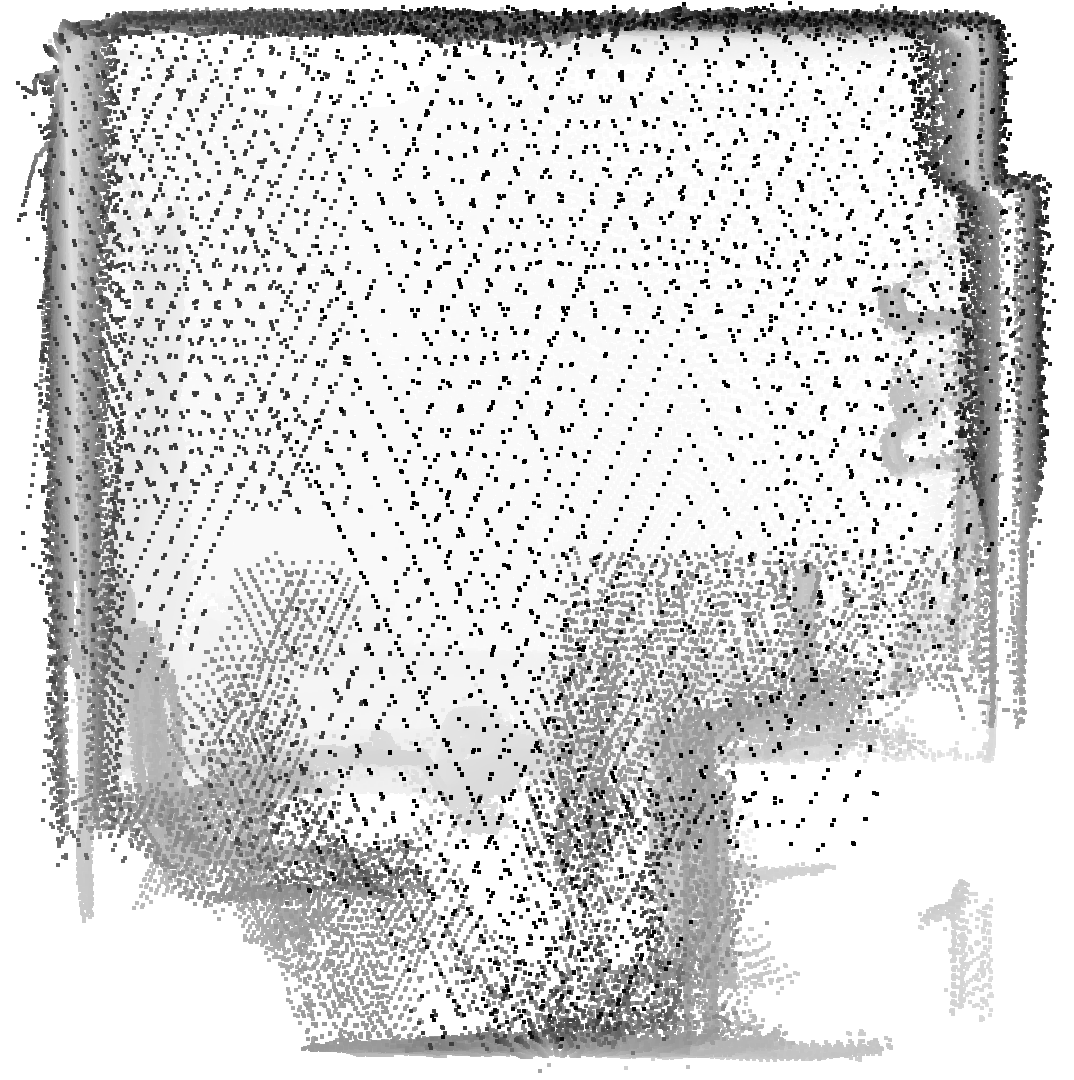
\includegraphics[width=\linewidth]{experimental_results/photos/z_bad_wall_grayscale.png}
        \caption{Before correction}
    \end{subfigure}
    \hfill
    \begin{subfigure}{0.46\linewidth}
        \centering
        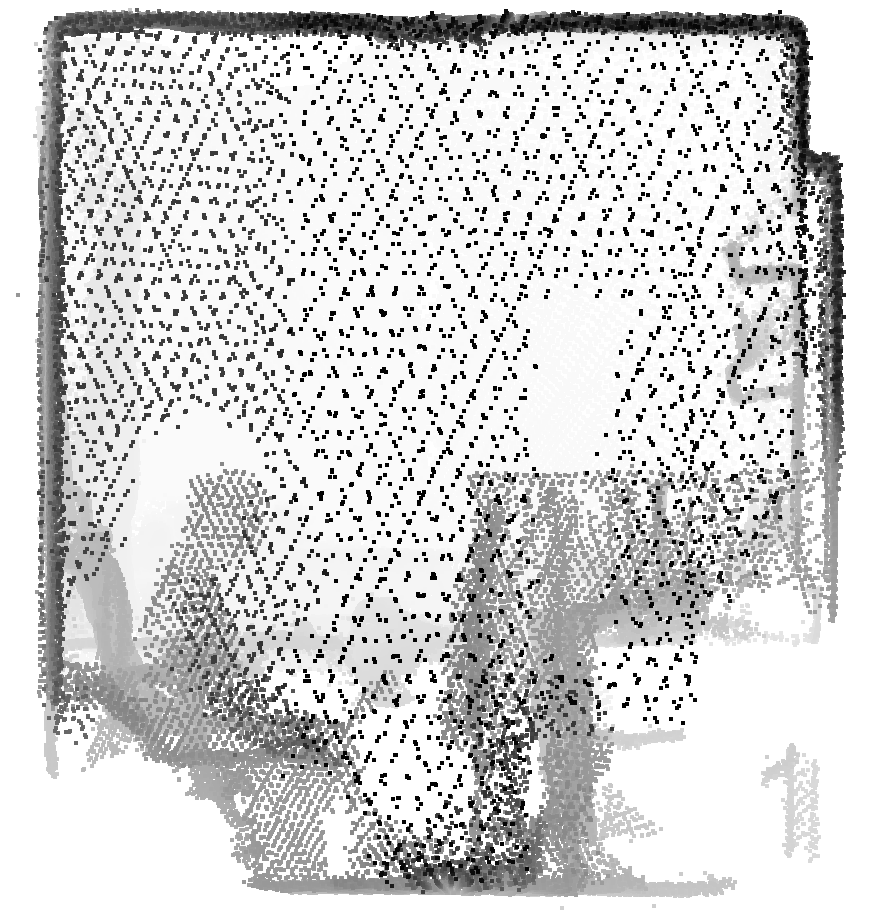
\includegraphics[width=\linewidth]{experimental_results/photos/z_good_wall_grayscale.png}
        \caption{After correction}
    \end{subfigure}
    \caption{Correction of the wall misalignment shown in side view}
\end{figure}

\subsection{Comparison with Photograph}
For this demonstration, the size of surfels in the Open3D visualisation window was set to maximally large in order to make the point cloud more visible and give a feeling of the continuity of surfaces.
\begin{figure}[H]
    \centering
    \begin{subfigure}{0.99\linewidth}
        \centering
        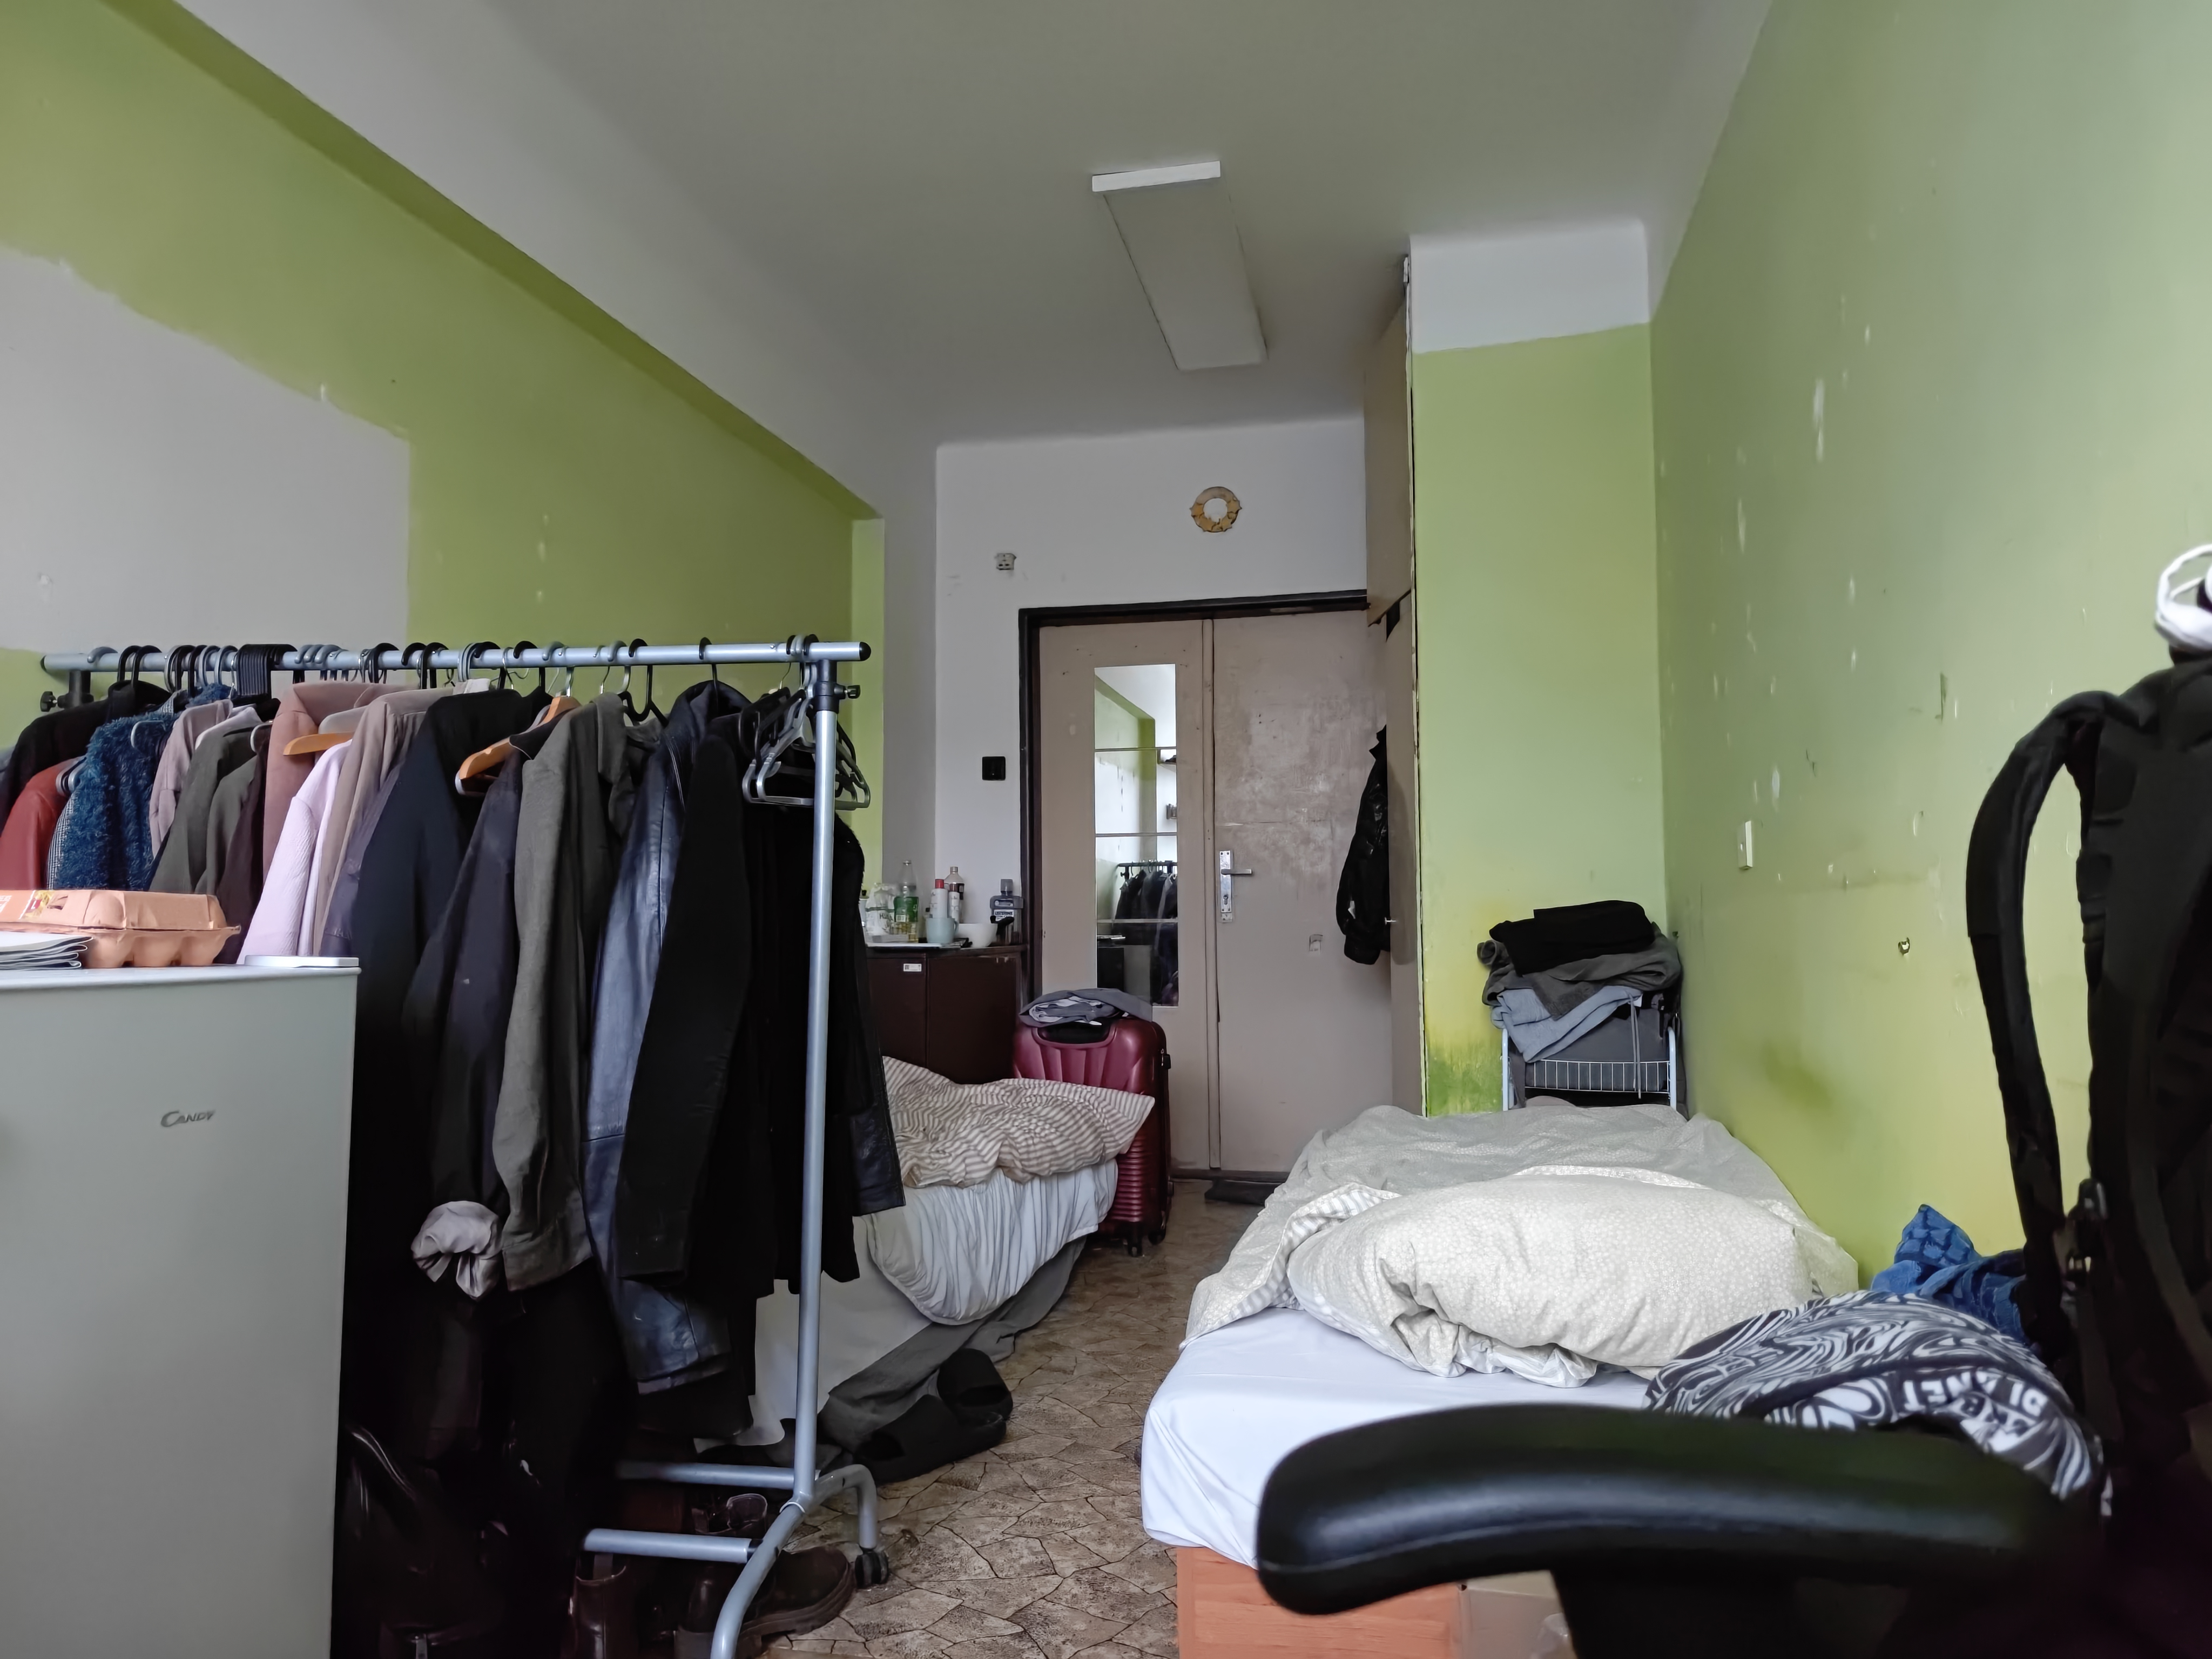
\includegraphics[width=\linewidth]{experimental_results/photos/room_photo.jpg}
        \caption{Photo}
    \end{subfigure}
    \hfill
    \begin{subfigure}{0.99\linewidth}
        \centering
        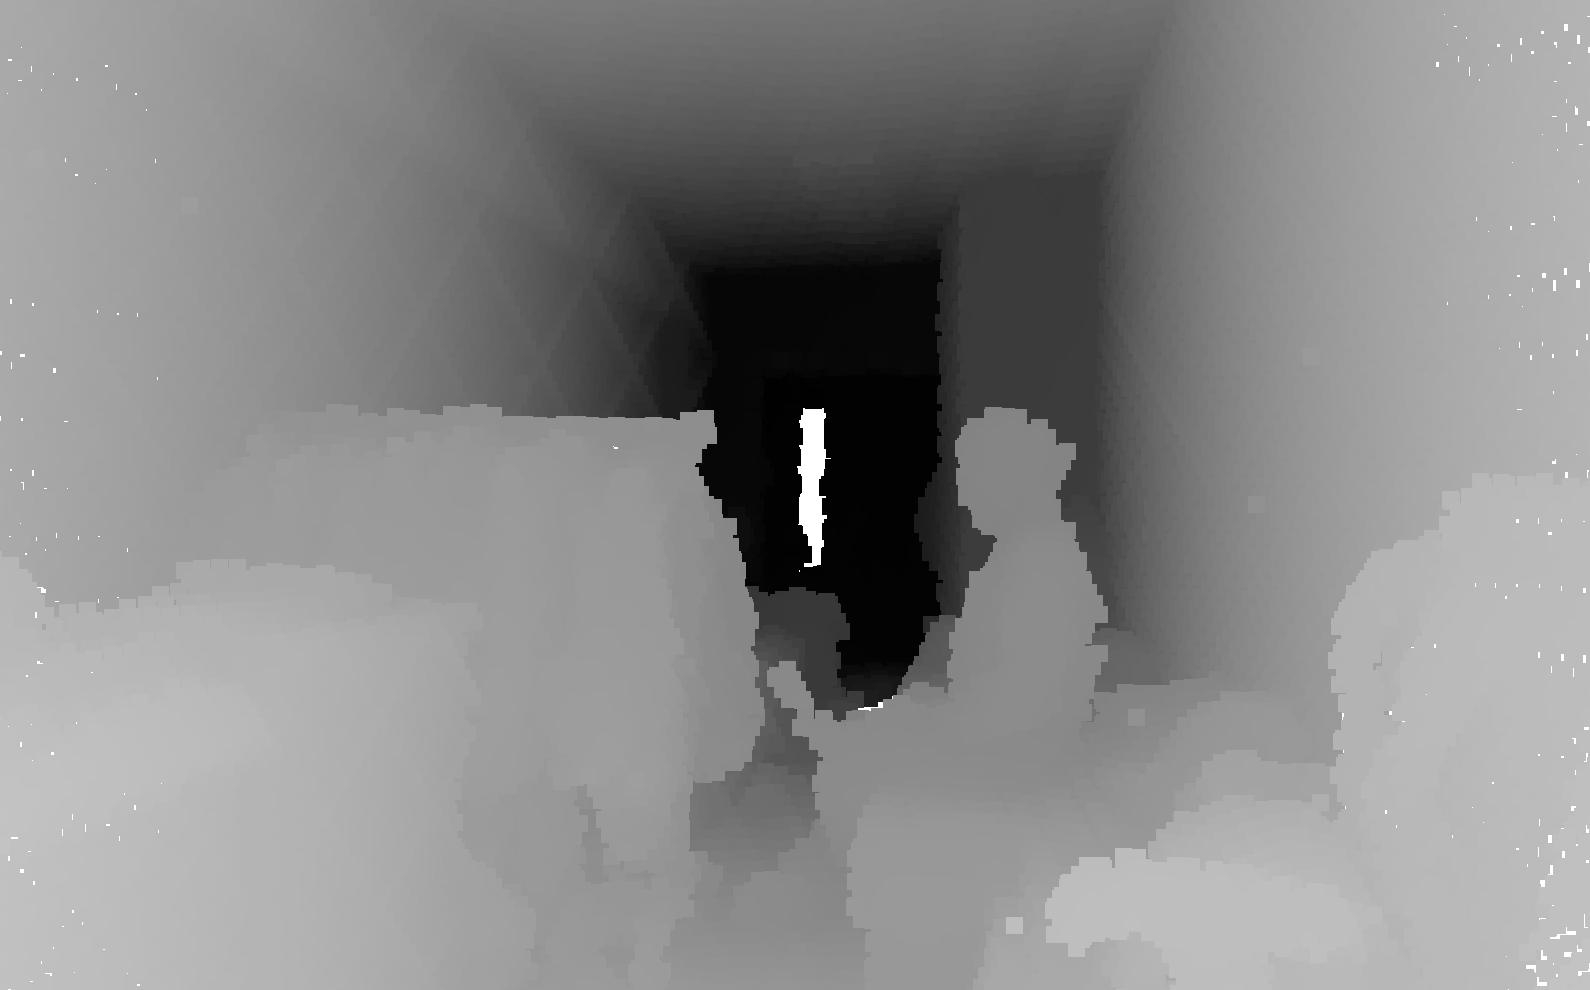
\includegraphics[width=\linewidth]{experimental_results/photos/z_room_pcd_grayscale.png}
        \caption{Point cloud}
    \end{subfigure}
    \caption{Comparison between a photo and the point cloud of a scanned room}
\end{figure}
Grayscale depicts the depth of the points, with darker points being farther away. Author is visible sitting on a bed. Points which were reflected by mirror were positioned at a greater distance due to the reflection of the \gls{lidar} beam and were therefore filtered out by the outlier removal process.